\documentclass[12pt,a4paper]{article}
\usepackage[utf8]{inputenc}
\usepackage[T1]{fontenc}
\usepackage{amsmath}
\usepackage{textcomp}

\usepackage{geometry}
\geometry{a4paper,left=25mm,right=25mm, top=2cm, bottom=2cm} 

\usepackage{graphicx} %fuer bilder

\usepackage{verbatim}




 \usepackage{mathptmx}
 \usepackage[scaled=.90]{helvet}
 \usepackage{courier}



\usepackage{listings}
\usepackage{color}
 
\definecolor{dkgreen}{rgb}{0,0.6,0}
\definecolor{gray}{rgb}{0.5,0.5,0.5}
\definecolor{mauve}{rgb}{0.58,0,0.82}

\pagestyle{empty}
\lstset{numbers=left, language=VHDL}
\lstset{showstringspaces=false,
basicstyle=\ttfamily\footnotesize,
breaklines=true,
tabsize=3,
commentstyle=\color{dkgreen},      % comment style
inputencoding={ansinew},
title=\lstname %zeigt titel der datei an
}

\usepackage{pdfpages} % fuer pdfs
\usepackage{hyperref} % fuer url


%keine einrückungen bei absatz
\parindent 0pt

\begin{document}
\title{Übung 05}
\author{Reinhard Penn, Bernhard Selymes, Robert Zeugswetter}
\date{Jänner 2016}

\normalsize


%Beginn des Dokuments

\newcommand{\Uebung}{Power}
\newcommand{\srcpath}{../../src}
\newcommand{\simpath}{../../sim}
\newcommand{\synpath}{../../syn}

%Angabe
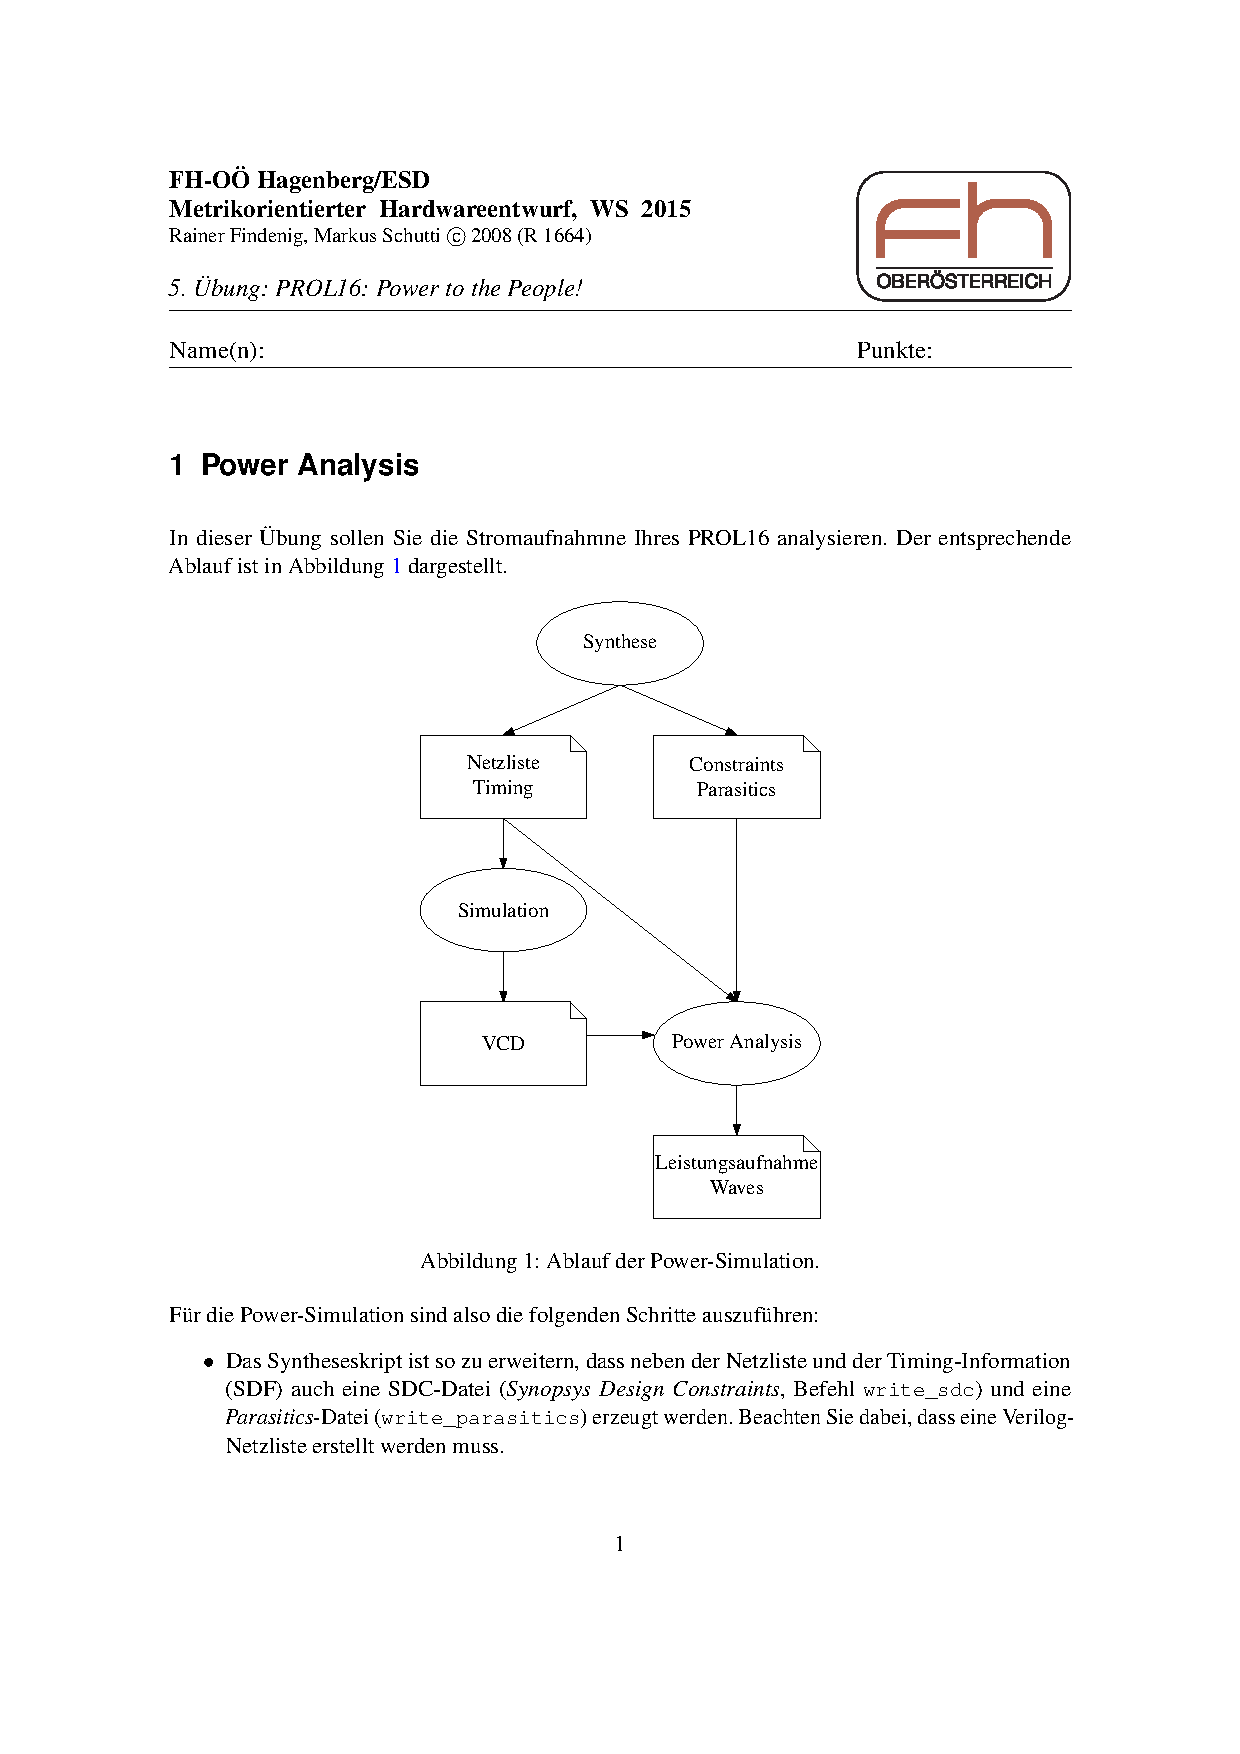
\includepdf[pages=-]{../Angabe.pdf}

\begin{center}
PROL16: Power Analyse und Optimierung\\
Übungsprotokoll zur Übung 5\\
Metrikorientierter Hardwareentwurf\\
Bernhard Selymes, Reinhard Penn, Robert Zeugswetter\\
11.01.2016
\end{center}

\section{Power Analysis}
Im Report, der durch \texttt{report\_power} erzeugt wird, wird der Stromverbrauch angegeben. Es wird angezeigt in welchen Hierarchieebenen wie viel Strom verbraucht wird und welche Art von Strom fließt. Der Gesamtverbrauch sind 557 uW wobei der Datenpfad 81.5 \% davon verbraucht und der Kontrollpfad 18.1 \%.

\section{Clock Gating}
Erklärung der Ausgabe von \texttt{report\_clock\_gating}: Die Register \texttt{RegTmpA/RegTmpB} bekommen kein Clock Gating, weil sie kein Enable-Signal haben. Die Register \texttt{Carry/Zero} haben schon Enable-Signale, aber sind jeweils nur ein Bit breit und bekommen wahrscheinlich daher kein Clock Gating.

Danach wurde der Befehl :
\begin{verbatim}
set_clock_gating_style 
  -sequential_cell latch 
  -positive_edge_logic {and} 
  -negative_edge_logic {or}
\end{verbatim}
gesetzt. Für die Register \texttt{Carry/Zero} wird nun Clock Gating verwendet.

Ungated Register (Ausschnitt):
\begin{verbatim}
-------------------------------------------------------------------
                     Ungated Register Report
-------------------------------------------------------------------
        Ungated Register     | enable | ctrl   | width  | removed
-------------------------------------------------------------------
datapath_inst/RegTmpB_reg_0_ |  NO    |  -     |  -     |  -
datapath_inst/RegTmpB_reg_1_ |  NO    |  -     |  -     |  -
\end{verbatim}

Zusammenfassung:
\begin{verbatim}
                    Clock Gating Summary
------------------------------------------------------------
|    Number of Clock gating elements    |        11        |
|                                       |                  |
|    Number of Gated registers          |     163 (81.91%) |
|                                       |                  |
|    Number of Ungated registers        |     36 (18.09%)  |
|                                       |                  |
|    Total number of registers          |        199       |
------------------------------------------------------------
\end{verbatim}

\subsection{Postlayout-Simulation}
Im Programm werden zuerst ein paar \texttt{nop}-Befehle ausgeführt und dann mit \texttt{loadi} ein Wert auf Register 1 geschrieben.

\begin{figure}[ht]
\centering
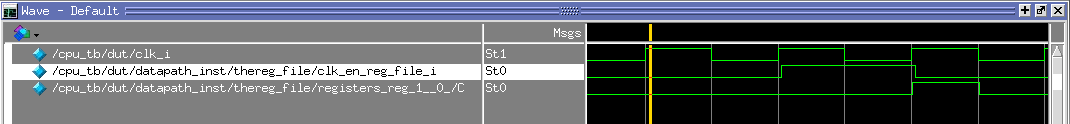
\includegraphics[width=\textwidth]{setregwave}
\caption{In dieser Abbildung ist die Waveform von den Signalen Global Clock, Clock Enable Regfile und der Clock von Register 1 Flip-flop 0 zu sehen.}
\label{fig_setregwave}
\end{figure}

\subsection{Power-Simulation}
Der Gesamtverbrauch sind 465 uW wobei der Datenpfad 80.7 \% davon verbraucht und der Kontrollpfad 18.9 \%. Die Implementierung mit Clock Gating verbraucht 16.5 \% weniger im Gegensatz zur Implementierung ohne Clock Gating. Die größte Einsparung ergibt sich beim Regfile, da dort die Register ohne Clock Gating immer neu geschrieben werden würden, auch wenn sie nicht verändert werden. Die kleinste Verbesserung ist bei der ALU, da diese ohnehin sehr viel arbeitet.

\subsection{Clock Gating und DfT}
Das Clock Gating verletzt die DfT-Regel, welche besagt, dass Clock Signale nicht gegated werden sollen. Der Clock muss immer aktiv sein, ansonsten kann es sein, dass die Scankette unterbrochen wird.



%\lstinputlisting[language=c]{../atpg_results.rep}
%\begin{lstlisting}
%  //detectable error
%  assign n148 = 0;
%  NAND30 U211 ( .A(n152), .B(n150), .C(alu_func_i[3]), .Q() );
%\end{lstlisting}

\end{document}
